\chapter{REFERENCIAL TEÓRICO}

\section{Manufatura Aditiva}
O princípio básico da manufatura aditiva (MA) é a 
capacidade de fabricar um modelo tridimensional "diretamente", não sendo
necessário o planejamento das operações de maneira individual e sim se preocupando
com as configurações como um todo.
O processo é calculado pelo fatiador com base em um modelo tridimensional digital,
geralmente criado a partir de \textit{Computer Aided Design} (CAD) e nas configurações do mesmo
e resulta nas intruções necessárias para a máquina de manufatura aditiva construir o modelo físico.
Uma das características 
principais da MA é a rapidez na qual é possível criar protótipo
diretamente de modelos digitais, por conta disso, em um contexto 
de desenvolvimento de produto, o termo prototipagem rápida era 
utilizado. Entretanto, conforme a MA foi se aperfeiçoando era 
perceptível a capacidade dessas tecnologias não só se aterem à 
produção de protótipos, mas também de peças utilizadas em 
produtos finais. Além disso, o termo não considerava o princípio 
básico que unia essas tecnologias e assim o termo manufatura 
aditiva foi apresentado e adotado pela \textit{American Society for 
Testing and Materials} (ASTM) \citeauthor{gibson15} (\citeyear{gibson15}).

Apesar da manufatura aditiva ter sido criada a mais de 30 anos, apenas
a partir de 2009, quando a última patente mais relevante de \textit{Fused Deposition Modeling} (FDM)
expirou. Com isso, vários entusiastas começaram a desenvolver essa tecnologia de uma
maneira "caseira", com o forte movimento RepRap. Por conta dessa característica
"caseira" e um senso de comunidade, os desenvolvimentos em sua maioria eram
de caráter \textit{Open Source} e com uma mentalidade de acessibilizar essa tecnologia para as pessoas.
Com os avanços tecnologicos feitos pela comunidade, empresas, pessoas e a mídia começaram
a se interessar cada vez mais, aumentando a popularidade das impressoras 3D e por consequência
trazendo muita atenção para a manufatura aditiva, que a partir dai, mais pesquisas, mais
empresas se interessavam em desenvolver esse tipo de tecnologia, não somente FDM \cite{attaran17}.

Atualmente, existe uma grande variedade de tecnologias e processos de manufatura aditiva.
Estes variam na maneira com que depositam o material, nos principios físicos que utilizam e nos materias
que podem ser utilizados. Como mencionado anteriormente, um dos métodos de manufatura aditiva mais populares
é a tecnologia FDM, entretanto existem diversas outras tecnologias que tem crescido muito em popularidade
como as tecnologias baseadas na cura seletiva de resinas, \textit{stereolithography} (SLA) e \textit{Masked stereolithography Apparatus} (MSLA),
alem de outras tecnologias menos acessíveis, mas com aplicações em diversas industrias, como por exemplo
\textit{selective laser melting} (SLM) e \textit{selective laser
sintering} (SLS) \cite{bikas16}.  

\begin{figure}[!htb]
    \begin{center}
    \caption{teste}
    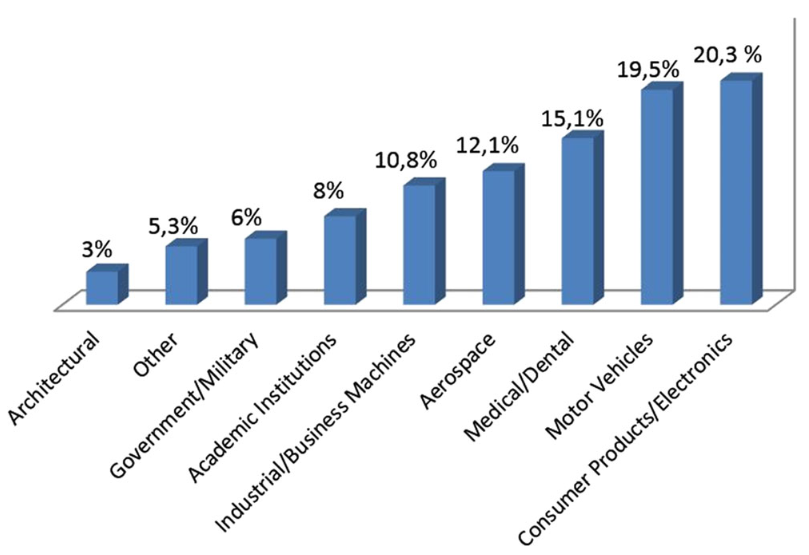
\includegraphics[scale=0.6]{bikas15industries}

    {\footnotesize Fonte: \citeauthor{bikas16}, \citeyear{bikas16}}
    \label{fig:label}
    \end{center}
\end{figure}

\ref{fig:label} figura

\section{\textit{Fused Deposition Modeling}}
\textit{Fused Deposition Modeling} (FDM) ou \textit{Fused Filament Fabrication} 
(FFF) é uma das tecnologias MA mais populares como mencionado anteriormente.
Ela se consiste por depositar material através de um processo 
onde um filamento de material é forçado dentro de uma câmara através,
geralmente, de rolos dentados onde em uma região específica esse 
material é liquefeito. Por conta da pressão criada pelo filamento 
adentrando a câmara, ainda no estado sólido como um pistão, 
o material liquefeito é extrudado através de um bocal, 
comumente fabricado de bronze. Então, o filamento liquefeito é 
depositado em uma plataforma de forma a percorrer a trajetória 
desejada utilizando mecanismos movidos de forma controlada, 
geralmente por motores de passos. O processo é repetido camada 
por camada, de forma que elas estejam apoiadas por camadas 
anteriores e a primeira camada continue fixa na plataforma ou 
cama, até que o processo finalize (TURNER et al., 2014) \cite{turner14}.

O trabalho de \cite{vyavahare20} apresenta algumas 
características sobre o desenvolvimento científico sobre 
FDM ao longo dos anos, tendo como base 211 artigos diferentes 
de 1994 a 2020. É apresentado um grande salto no número de 
artigos publicados no tema em anos recentes (2015 a 2018) 
(Figura 1), com 56\% dos temas trabalhados em torno da 
otimização de parâmetros de impressão, acompanhado de 17\% de 
trabalhos relacionados a aplicações utilizando o processo FDM, enquanto apenas x\%
são relacionados a outros temas, incluindo avanços tecnologicos relacionados
a melhorias de \textit{hardware} e \textit{software} desses dispositivos.
(Figura 2).

\begin{figure}[!htb]
    \centering
    \caption{teste}
    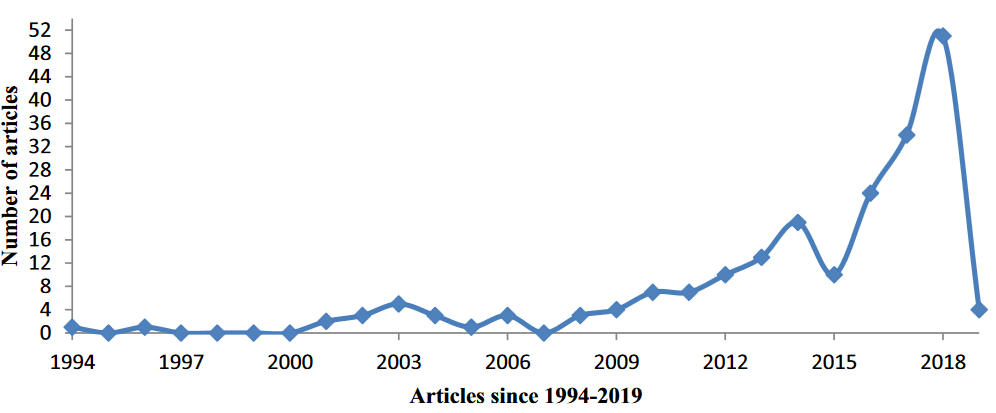
\includegraphics[scale=0.5]{vyan20npub}
    
    {\footnotesize Fonte: \citeauthor{vyavahare20}, \citeyear{vyavahare20}}
    \label{fig:label2}
\end{figure}

\begin{figure}[!htb]
    \centering
    \caption{teste}
    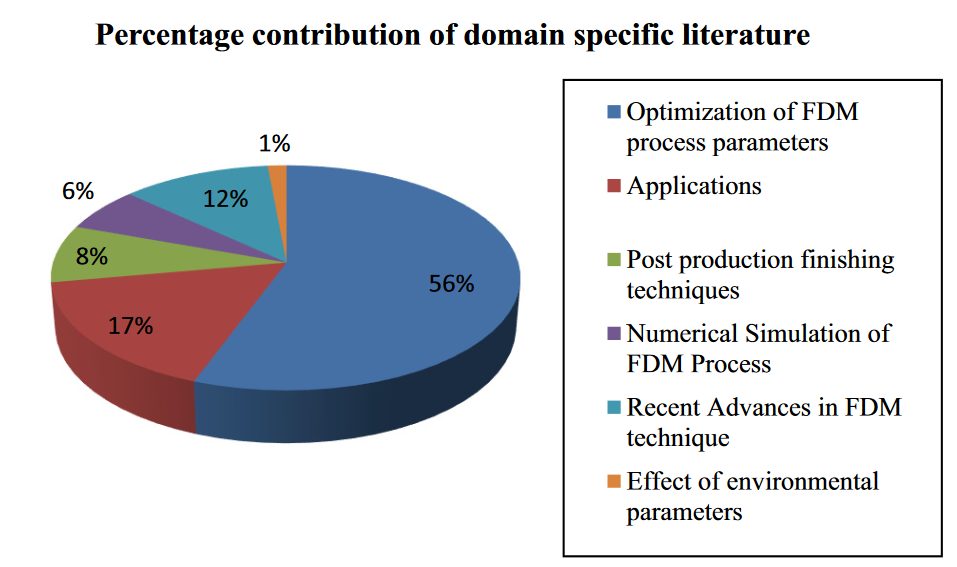
\includegraphics[scale=0.5]{vyan20oizzama}

    {\footnotesize Fonte: \citeauthor{vyavahare20}, \citeyear{vyavahare20}}
    \label{fig:label3}
\end{figure}

\ref{fig:label} figura

Podemos separar, de maneira simplificada, a porção de software de impressoras 3D
FDM em três principais etapas: fatiamento (\textit{slicing}), geração de comando e controle.
A etapa de fatiamento involve a topologia e a criação de instruções a partir do modelo,
é nessa fase onde se decide a sequência de movimentos e outros eventos.
Já na etapa de geração de comando, as instruções criadas pelo fatiador (\textit{slicer}) na etapa anterior
são interpretadas e os comandos detalhados são gerados, por exemplo as curvas de velocidade.
Esses comandos são utilizados para movimentar os motores e outros equipamentos da impressora.
Na etapa de controle, uma etapa relativamente nova nas impressoras 3D mais acessíveis, 
tecnicas de controle são utilizadas para se diminuir vibrações e variações indesejadas em quaisquer
parâmetros controlados, como a temperatura do bico. Um dos grandes avanços nessa etapa
foi a implementação da técnica de \textit{Input Shaping} por um \textit{firmware Open Source} de impressora 3D chamado Klipper.
Após a inclusão dessa etapa, principalmente no controle dinâmico da impressora, as capacidades
de velocidades e qualidade chegaram a outro patamar se comparados a impressoras que não implementam essa etapa \cite{klipperdoc}.
% \subsection{Five-phase S-curve Velocity Model}

\subsection{Feedforward}
Dentre os métodos de controle em aplicações FDM o \textit{Feedforward} 
é o mais eficiênte dada as limitações de custo em impressoras 
3D comuns e é capaz de ter um impacto maior em sistemas 
conhecidos e sensíveis ao erro, onde buscam corrigir o erro 
antes que ele aconteça. O método de \textit{feedback} é mais eficiente em
diminuir o impacto de excitações externas ou desconhecidas,
entratanto não consegue prever os efeitos do sistema, se encaixando
melhor em aplicações de usinagem utilizando CNCs (\textit{Computer Numerical Control}),
onde o valor dos equipamentos é maior e as forças envolvidas no corte
influênciam mais do que as vibrações do próprio sistema.
Já no caso das impressoras, quase 100\% dos efeitos é causado pelo próprio
sistema. As principais limitações da aplicação de técnicas Feedforward
em impressoras 3D são a dificuldade de montar um modelo representativo,
a exigência computacional elevada e por fim a necessidade da simulação
se extender do incio ao fim, pela dependência de se basear no estado 
incial da impressão \cite{ramani20,duan18}.

\subsubsection{\textit{Input Shaper}}
Conhecendo a trajetória desejada e conhecendo características 
do sistema é possível computar os comandos fornecidos para 
calcular uma série de comandos, levando em consideração as 
características do sistema para que o comando de referência 
seja modificado de forma à trajetória final ser o mais próximo 
possível do comando de referência. Entretanto, ao invés de 
computar todo o comando de referência, é possível obter um 
comando modificado em tempo real através de um filtro. 
Uma das abordagens desse tipo de filtro de comando é o 
\textit{Input Shaper}, onde variados \textit{Shapers} são construídos levando 
em consideração diferentes objetivos e restrições 
\cite{singhose97}.

\begin{figure}[!htb]
    \centering
    \caption{teste}
    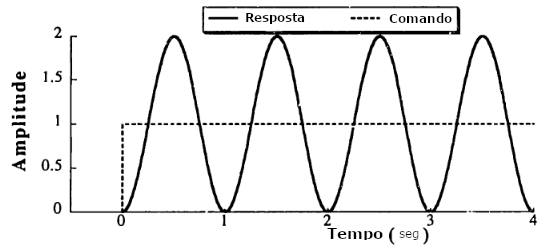
\includegraphics[scale=0.5]{inputshaperstepresponse1order}
    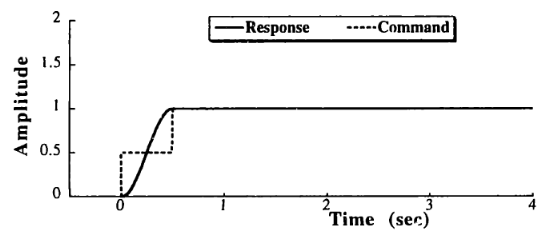
\includegraphics[scale=0.5]{inputshaperstarcasepresponse}

    {\footnotesize Fonte: \citeauthor{singhose97}, \citeyear{singhose97}}
    \label{fig:label4}
\end{figure}

Essa abordagem vem sendo explorada na comunidade "faça você mesmo" a partir de 2017 
quando a última patente desse método expirou, e tem aprimorado a área como
um todo, empurrando os limites anteriores de velocidade e precisão,
sendo popularizada pelo Klipper \cite{klipperkinematic}.


\begin{figure}[!htb]
    \centering
    \caption{teste}
    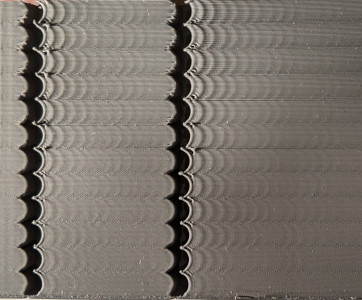
\includegraphics[scale=0.6]{ringing-test}

    {\footnotesize Fonte: \citeauthor{klipperkinematic}, \citeyear{klipperkinematic}}
    \label{fig:label4}
\end{figure}

\subsubsection{filtered basis function (FBF)}
O método FBF necessita que a trajetória a ser rastreada seja totalmente
conhecida e que a trajetória controlada possa ser expressa como
uma combinação linear de funções base possuindo coeficientes desconhecidos.
As funções base são utilizadas em um controle feedforward utilizando
o modelo dinâmico do sistema e selecionando os coeficientes de maneira a
minimizar os erros dada uma trajetória desejada.
\cite{ramani17}

\begin{figure}[!htb]
    \centering
    \caption{teste}
    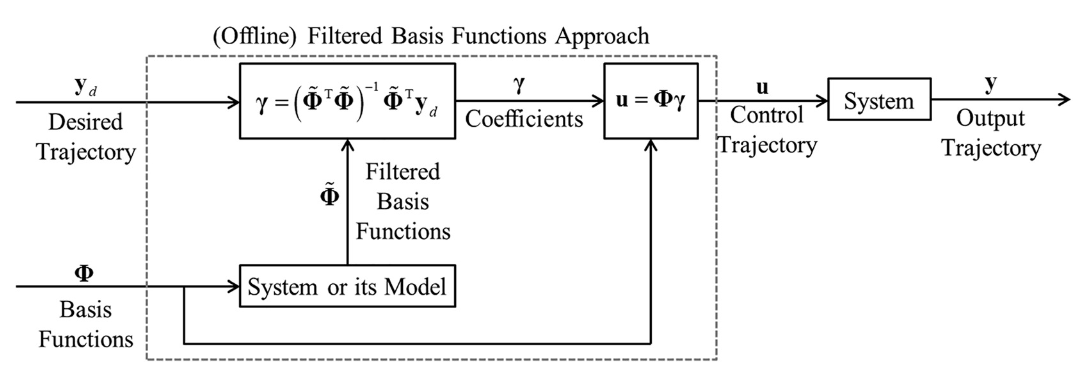
\includegraphics[scale=0.5]{ramani17blockfbf}

    {\footnotesize Fonte: \citeauthor{ramani17}, \citeyear{ramani17}}
    \label{fig:label7}
\end{figure}

\subsubsection{\textit{Limited-preview filtered B-splines}}
Uma das maiores dificuldades que os métodos avançados para o
controle \textit{feedforward} de trajetórias é a necesidade de se conhecer
completamente a trajetória desejada, o que implica em um grande custo
computacional, principalmente em situações onde são necessárias uma
grande quantidade de amostras da trajetória, por exemplo em casos de alta resolução
e casos de longa duração.
O \textit{limited-preview filtered B-splines} divide a trajetória desejada em subgrupos
com um número menor de amostras e utiliza um algorítmo de \textit{receiding horizon} para
calcular recursivamente os coeficientes da função B-spline que minimizam os erros
de trajetória \cite{duan18}.

A partir dessa otimização da divisão da trajetória em subgrupos, esse método
conseguiu ser testado utilizando uma impressora 3D de verdade com modelos simples.
Apresentando resultados promissores apresentados na figura \ref{fig:duancubo}.

\begin{figure}[!htb]
    \centering
    \caption{teste}
    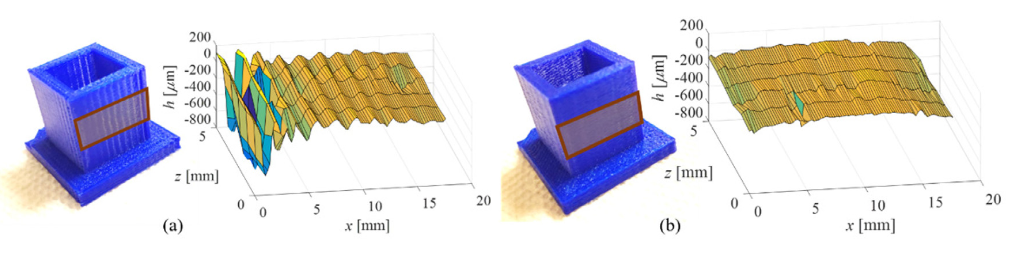
\includegraphics[scale=0.5]{duancubo}

    {\footnotesize Fonte: \citeauthor{duan18}, \citeyear{duan18}}
    \label{fig:duancubo}
\end{figure}

\subsubsection{\textit{Robust Filtered Basis Functions}}

However, the FBF approach faces at least two practical chal-
lenges. The first is that its computational cost becomes very
high as the length (number of samples) in the motion trajectory
increases. To overcome this challenge, a limited preview version
of FBF, viz., limited preview filtered B-splines (LPFBS), was
proposed by Duan et al. [11]. LPFBS was shown to significantly
reduce the computational cost of the FBF approach without
significantly sacrificing its tracking performance, allowing it to
be implemented successfully on a desktop 3-D printer [11]. A
second challenge is that, being a purely feedforward technique,
the tracking accuracy of the FBF approach degrades in the
presence of inaccuracies in the plant model or uncertainty in
the plant dynamics [11].
In the presence of uncertainty in the plant dynamics, the
tracking accuracy of feedforward controllers such as FBF can be

solution, which facilitates LPFBS, is needed.
Hence, this article (and its preliminary version [28]) makes
the following contributions to the literature.
1) It proposes a robust FBF approach that retains the ele-
gance of the least-squares solution of the standard FBF
approach by using a robust filter instead of nominal plant
dynamics to filter basis functions.
2) It proposes the inverse of an optimal feedforward con-
troller that minimizes an error cost function for known
plant uncertainty as a robust filter for use in robust FBF.
3) It demonstrates the effectiveness of the proposed robust
FBF approach using simulation examples and experi-
ments on a desktop 3-D printer with dynamic uncertainty.
\cite{ramani20}


\begin{figure}[!htb]
    \centering
    \caption{teste}
    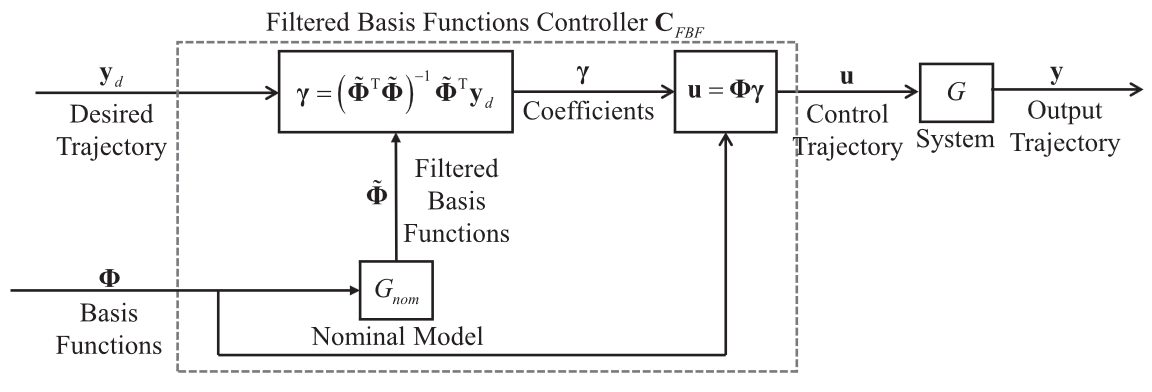
\includegraphics[scale=0.5]{ramani20blockfbf}

    {\footnotesize Fonte: \citeauthor{ramani20}, \citeyear{ramani20}}
    \label{fig:label9}
\end{figure}

\section{Geração de comando}
A geração de comando é o processo que coordena a ativação dos 
atuadores, motores, dentre outros componentes de uma impressora. 
Ele recebe como base uma série de comandos que precisam ser 
interpretados e interpolados. Esse processo é responsável pelo 
controle de velocidade, aceleração dentre outras atividades que 
variam no tempo \cite{yu20}. 

\subsection{\textit{Look ahead}}
No processo de impressão 3D são fornecidos para a impressora 
uma sequência de pontos no espaço e limitações de velocidade 
entre os mesmos. A velocidade nos pontos é compartilhada entre 
trajetos em sequência, o que torna considerá-los 
independentemente ineficiente, introduzindo aceleração e 
desaceleração desnecessária impactando negativamente no tempo 
de impressão e na qualidade da peça impressa.
O algoritmo \textit{Look Ahead} procura manter o máximo de velocidade 
possível entre movimentos distintos, evitando acelerações e 
desacelerações desnecessárias, apesar de ser necessário um 
pré-processamento desses pontos que introduzem um custo 
computacional maior (YU et al. 2020) \cite{yu20, klipperkinematic}.

\subsection{Curvas de velocidade trapezoidal}
As impressoras 3D entre outros equipamentos, como máquinas CNC, necessitam
de um planejamento de velocidade, pois o Gcode fornece apenas as velocidades desejadas
de cada movimento, enquanto o algorítmo de lookahead calcula as velocidades
de junção entre os movimentos, portanto ainda se faz necessário planejar
o comportamento da velocidade ao longo do tempo do trajeto entre a velocidade incial
e final do movimento.
Uma das maneiras mais simples para a criação dessa curva de velocidade é
a criação de uma curva trapezoidal, onde podemos separar o setor em 3 segmentos
de aceleração constante. Em um primeiro momento uma crescente de velocidade até
a velocidade desejada, seguido de um segmento de velocidade constante e por fim
um segmento de desaceleração constante até a velocidade final.
Alguns ajustes são feitos para as diferentes condições de velocidade inicial, final e
velocidade máxima atingida com uma determinada aceleração máxima, que pode
fazer com que se diminua a quantidade de segmentos \cite{yu20,klipperkinematic}.

\begin{figure}[!htb]
    \centering
    \caption{teste}
    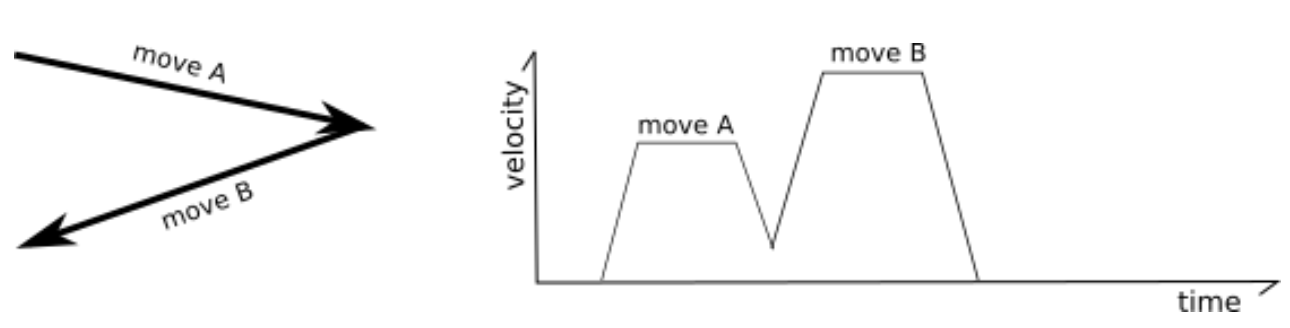
\includegraphics[scale=0.3]{lookaheadboth2}

    {\footnotesize Fonte: \citeauthor{klipperkinematic}, \citeyear{klipperkinematic}}
    \label{fig:label9}
\end{figure}

\begin{figure}[!htb]
    \centering
    \caption{teste}
    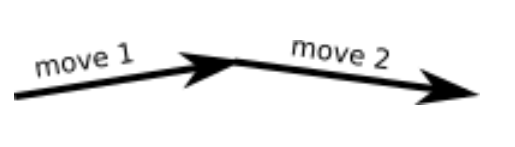
\includegraphics[scale=0.3]{lookaheaddir1}
    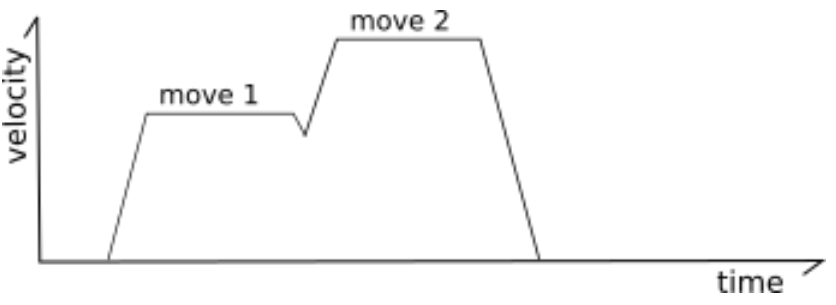
\includegraphics[scale=0.3]{lookaheadtrap1}

    {\footnotesize Fonte: \citeauthor{klipperkinematic}, \citeyear{klipperkinematic}}
    \label{fig:label9}
\end{figure}


\begin{figure}[!htb]
    \centering
    \caption{teste}
    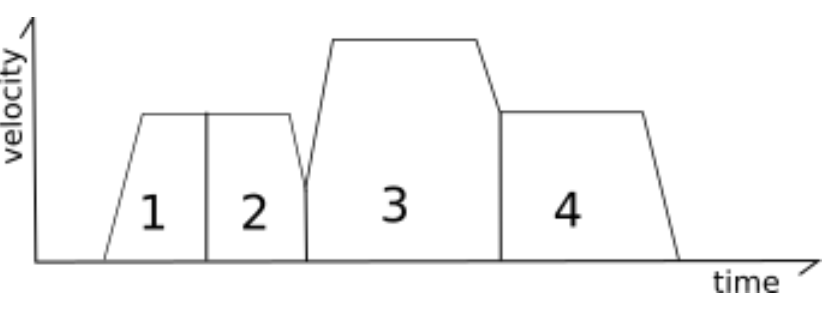
\includegraphics[scale=0.4]{trapezoidex}

    {\footnotesize Fonte: \citeauthor{klipperkinematic}, \citeyear{klipperkinematic}}
    \label{fig:label9}
\end{figure}


\subsection{Espaço de Estados}

A maioria dos sistemas dinâmicos pode ser escritos através de uma formulação
chamada de espaço de estados, que tem como objetivo expressar modelos 
de equações diferencias parciais (EDP) ou ordinárias (EDO) de ordem superior
como um conjunto de EDPs ou EDOs de primeira ordem.
Essa formulação é construida a partir de um principio de autoregressão
das equações. Na equação \ref{eq:edo_ex} podemos observar uma EDO de segunda ordem representando
um sistema massa mola simples,
logo abaixo (\ref{eq:espaco_de_estados_ex}) a mesmsa equação representada na formulação
de espaço de estados \cite{hamilton94}.

\begin{equation}
    \label{eq:edo_ex}
    m \ddot x+c \dot x+kx = f(t)
\end{equation}

\begin{equation}
    \label{eq:espaco_de_estados_ex}
    \begin{bmatrix}
        \dot x \\
        \ddot x
    \end{bmatrix}
    =
    \begin{bmatrix}
        0 & 1 \\
        k/m & c/m
    \end{bmatrix}
    \begin{bmatrix}
        x \\
        \dot x
    \end{bmatrix}
    +
    \begin{bmatrix}
        0 \\
        1
    \end{bmatrix}
    f(t)
\end{equation}

\subsubsection{Runge-Kutta}
Runge Kutta é um algoritimo de integração numérica baseada na série de Tailor onde,
nas formulações explicitas são calculados 4 coeficientes que são utilizados para estimar
o próximo ponto, assim caracterizando um algoritmo iterativo de valor inicial \cite{bettis79,dormand80}.

\subsection{\textit{Objective Function Optimization}}
Funções objetivo de otimização são elementos importantes na execução de algoritimos
de otimização. Alguns estudos apontam que a qualidade e o número de variáveis de
projeto cruciais para o resultado da otimização, além disso outros sub-parâmetros
também são relevantes como restrições, limites e valores iniciais. A coerência entre
estes fatores depende abilidade e de uma visão abrangente de seu criador \cite{albaghdadi21}.

